\chapter{Metodologia}

\section{Gerência do Projeto}

Para realizar a gerência do projeto Hedwig, foram usadas certas diretrizes do PMBOK \cite{pmi} e da norma ISO/IEC 12207 \cite{iso12207} como referência para coordenar os processos.

\subsection{Gerência de Escopo}

Segue a EAP (Estrutura Analítica do Projeto), que orientou as entregas realizadas e escopo do projeto.

\begin{figure}[H]
	\centering
	\caption{EAP do Hedwig}
	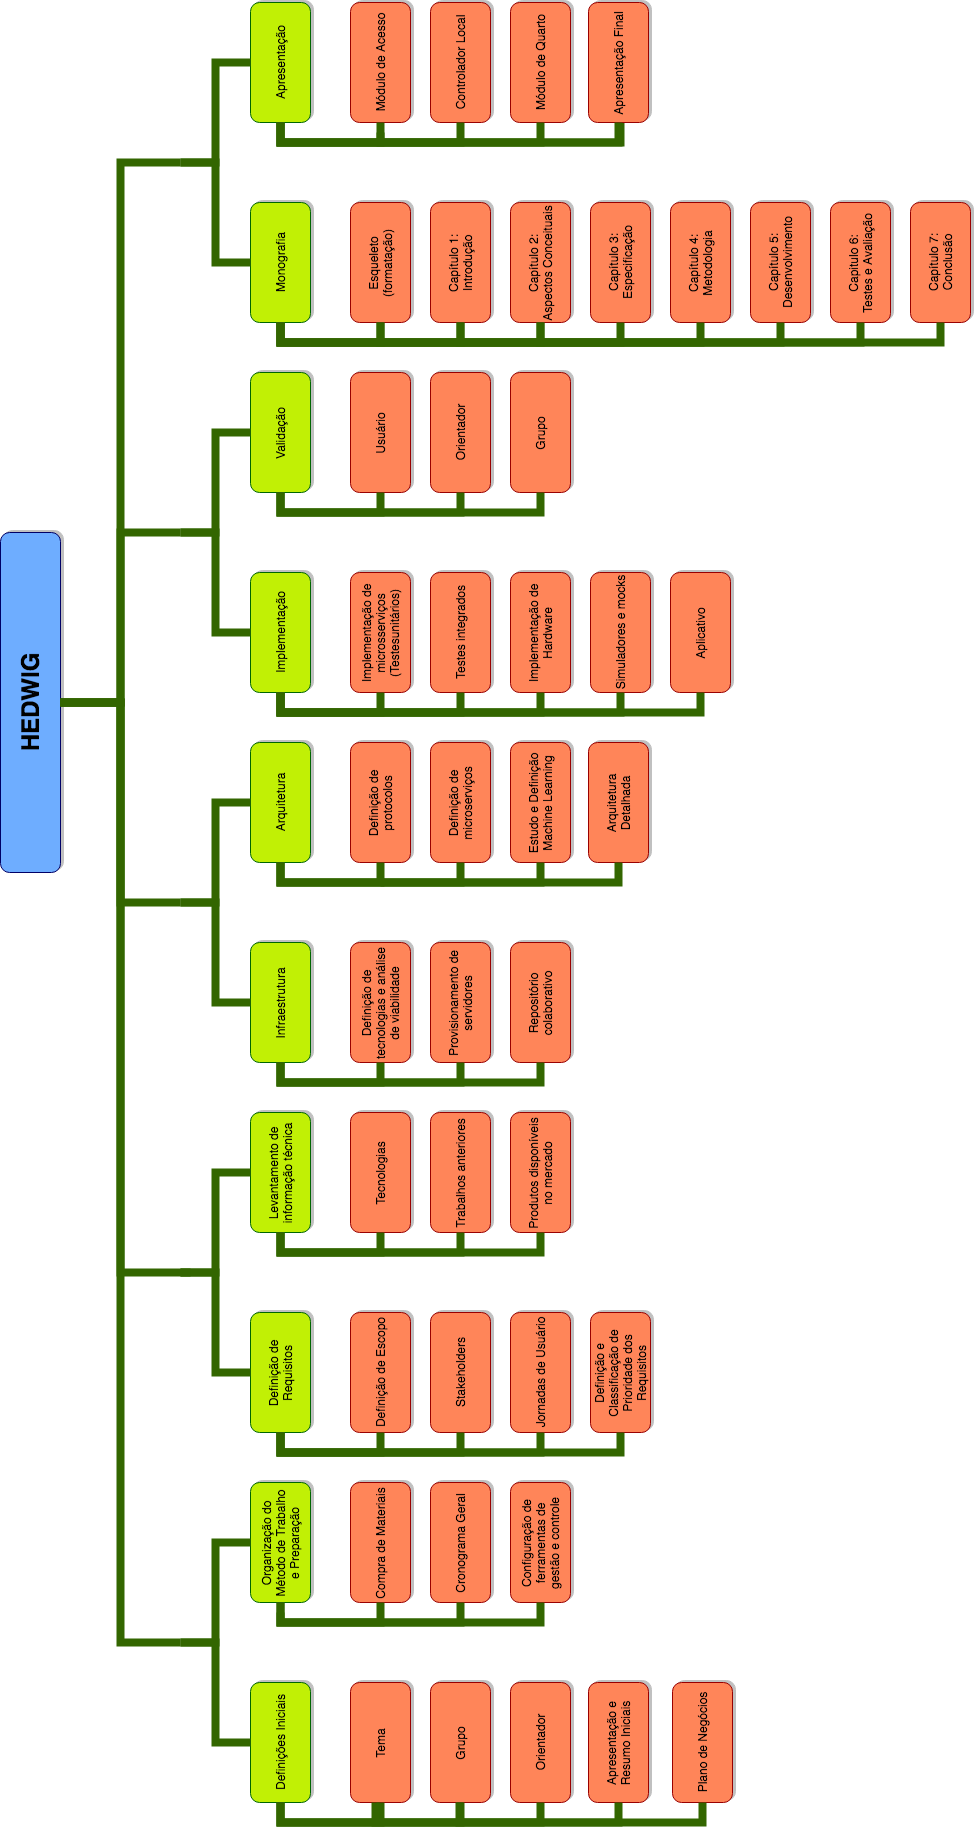
\includegraphics[width=0.8\textwidth]{Hedwig_EAP}
	\label{fig:Hedwig_EAP}
\end{figure}

\subsection{Gerência de Aquisição}

O gerenciamento de aquisições envolve primariamente a compra dos materiais necessários para implementação dos módulos físicos. Foi necessário analisar o que adquirir e como fazê-lo, levando em consideração as limitações de tempo do projeto --- a demora ou atraso na entrega dos componentes eletrônicos causaria um atraso no cronograma. A escolha dos fornecedores priorizou, então, o custo e o prazo de entrega.

A relação de materiais necessários para a confecção de um módulo básico encontra-se no Anexo \ref{listamateriais}.

\subsection{Gerência de Processos de Software}

Para gerenciar o código-fonte e permitir o trabalho da equipe em múltiplas partes do projeto ao mesmo tempo, foi utilizado o Git, um sistema de controle de versão distribuído. Para publicação do código, foi escolhido o GitHub, onde criou-se a organização Hedwig\footnote{https://github.com/hedwig-project} e os repositórios que contém o código das diversas partes do sistema. A preferência pelo GitHub se deu pelas suas funcionalidades de gerenciamento e colaboração, como a notificação de \emph{bugs}, acompanhamento do progresso de tarefas e criação de \textit{wikis}, além de ser uma plataforma conhecida por abrigar grandes projetos \emph{open-source} que chegam a ter centenas ou milhares de contribuidores \cite{github}. O GitHub disponibiliza também uma ferramenta para armazenamento de \emph{Issues} --- atividades que necessitam ser observadas ou desenvolvidas em um projeto. Esse recurso foi essencial na organização de tarefas e rastreamento de mudanças em curso.

Para a coordenação de trabalho nesses repositórios, foi utilizado o fluxo conhecido como \textit{Feature Branch Workflow} \cite{atlassian}, caracterizado pela criação de \textit{branches} (ramificações) para o desenvolvimento de cada nova funcionalidade. Ao final do desenvolvimento de cada funcionalidade, é feito um pedido para mesclar à \textit{master branch}, ramificação principal, o código desenvolvido na ramificação atual --- conhecido como \emph{Pull Request}. A utilização de \emph{Pull Requests} promove maior controle sobre a atualização do código mantido, e também promove a revisão do código pelos aprovadores. 

Já outros tipos de documentação formal do sistema, como textos e planilhas, foram editados e armazenados no Google Drive\footnote{https://www.google.com/drive/}, ferramenta de armazenamento e backup da Google que também permite colaboração, compartilhamento e controle de versão.

\subsection{Gerência de Comunicação}

Para comunicar as tarefas, estudos e pesquisas sendo realizadas durante o projeto, foi utilizado o Trello\footnote{https://trello.com/}, um sistema online para organização de ideias e projetos, que permite listagem e acompanhamento das atividades a serem realizadas, permitindo a adição de prazos, delegação de responsáveis e categorização das tarefas.

Foram realizadas diversas reuniões online usando ferramentas de videoconferência, como o Google Hangouts\footnote{https://hangouts.google.com} e o Skype\footnote{https://www.skype.com}, que, além do \emph{streaming} de vídeo com áudio, possuem funcionalidades como mensagens de texto, envio de arquivo e compartilhamento de tela, facilitando demonstrações e testes integrados.

\subsection{Gerência de Riscos}

Para gerenciar os riscos do projeto, foram realizadas reuniões periódicas com participação das partes interessadas --- grupo e orientadores --- nas quais discutiam-se táticas de análise, planejamento e monitoramento. Nessas sessões, foi possível identificar riscos por meio da revisão da documentação e de técnicas de \emph{brainstorming} e definir estratégias de abordagem de riscos.

\section{Pesquisa Bibliográfica}

O estudo dos tópicos relacionados a aprendizagem de máquina foi realizado com auxílio do curso \emph{Aprendizagem Automática}, do Professor Andrew Ng\footnote{ https://www.coursera.org/learn/machine-learning}, oferecido pela Universidade de Stanford e disponibilizado no Coursera, uma plataforma de MOOCs (\textit{Massive Open Online Courses}) que oferece cursos abertos e especializações.

Os cursos da especialização em \textit{Data Science} da Universidade Johns Hopkins\footnote{ https://www.coursera.org/specializations/jhu-data-science}, também disponíveis no Coursera, foram usados como referência e treinamento para realizar a coleta de dados de maneira metódica. Por esse motivo, foi dada maior atenção ao curso \textit{Getting and Cleaning Data}. Contudo, também foi aproveitado conteúdo do curso \textit{Practical Machine Learning}.

\section{Ferramentas e Tecnologias}

Para a aprendizagem da biblioteca React, para o desenvolvimento do \emph{front-end}, foi usada como referência a documentação oficial\footnote{https://facebook.github.io/react/docs/hello-world.html} oferecida pelo Facebook e o curso \textit{React for Beginners} de Wes Bos\footnote{ https://reactforbeginners.com/}. O aprendizado de Redux foi auxiliado pelo curso \textit{Learn Redux}\footnote{https://learnredux.com}, do mesmo autor. O conhecimento necessário à utilizaçãodo Spring Boot foi obtido com base no guia de referência oficial\footnote{https://docs.spring.io/spring-boot/docs/current/reference/htmlsingle/}.

\section{Método de Testes}

A estratégia de testes utilizada está fortemente relacionada com a estratégia de desenvolvimento. A implementação do projeto foi realizada em partes, segregadas de acordo a área de aplicação. Assim, as diversas frentes puderam ser desenvolvidas em paralelo, como os módulos, servidor local, aplicativo cliente, etc. juntamente com os seus respectivos testes.

Para cada tarefa específica foram efetuados testes unitários, de pequeno alcance, para validar a funcionalidade ou alteração. O desenvolvimento do servidor local contou também com testes unitários automatizados, entretanto sem cobertura do sistema inteiro. Para testes específicos dos \emph{endpoints} do servidor na nuvem foi utilizada a ferramenta Postman\footnote{https://www.getpostman.com/}, que permite simular requisições a tais \emph{endpoints}, configurando todos os parâmetros necessários e informações de cabeçalho HTTP, e apresenta ao usuário a resposta recebida.

Durante a integração das partes, houveram diversos testes ponto-a-ponto, para verificação do funcionamento completo do sistema. Utilizou-se para isso o Software MQTT Fx\footnote{http://mqttfx.jensd.de/}, onde é possível obter as mensagens encaminhadas pelo sistema de mensageria, e compará-las com os resultados esperados. Na Subseção \ref{testesTopicos} são mostrados alguns casos de testes utilizados durante a configuração do Broker Mosquitto, enquanto a seção \ref{atttestefimafim} contém um exemplo de teste fim a fim realizado com aplicativo, servidor local, nuvem e módulo.

Com a instalação do sistema em duas residências distintas, houve uma validação contínua de premissas e levantamento de requisitos, principalmente aqueles relacionados à usabilidade. Foram realizados diversos testes de conceito em campo, de forma que muitas soluções, embora fizessem sentido experimentalmente em implementações isoladas, não eram adequadas para módulos instalados em uma residência real. Ainda, atualizações e melhorias foram entregues frequentemente, contribuindo para o crescimento iterativo do projeto (destacam-se a aplicação dos princípios 2 e 4 do Agile Manifesto\footnote{http://agilemanifesto.org/iso/ptbr/manifesto.html}, que dissertam sobre mudanças frequentes de requisitos e entregas frequentes de software).

Em especial, o contato do desenvolvedor dos módulos com todos os problemas e desafios encontrados com o uso do sistema em sua residência facilitou sua proximidade com um dos stakeholders principais, possibilitando um \textit{feedback} rápido, reduzindo o ciclo de desenvolvimento consideravelmente.
